%======================== Kapitola: Součástky pro výkonovou elektroniku ============================
% !TeX spellcheck = cs_CZ
% librarian:
% file:///C:/wamp/www/Librarian/library/00138.pdf
\setchaptertoc
\chapter{Budiče IGBT a MOSFET tranzistorů}


  \section{Úvod}
    V obecném smyslu se pojmem budič výkonové součástky rozumí určité rozhraní mezi řídicí
    jednotkou a výkonovou součástkou. Základní funkcí je přizpůsobit logické řídicí signály způsobu
    ovládání hradla výkonové součástky. S rostoucím instalovaným výkonem a spínací frekvencí
    výkonového elektronického systému jsou na budiče kladeny vyšší nároky. Častým požadavkem je
    spínání výkonové součástky na plovoucím potenciálu vůči řídicímu signálu.
    Z toho vyplývá nutnost galvanického oddělení řídicích signálů na rozhraní mezi řídicími a
    výkonovými obvody elektronického systému.  Ve většině aplikací jsou také na galvanické oddělení
    kladeny ještě bezpečnostní požadavky. Můžeme se proto setkat s budiči, které mají řídicí signály
    galvanicky odděleny, ačkoliv výkonový spínač pracuje na stejném potenciálu jako řídicí
    elektronika, nebo například s budiči s dvojitou izolací.

    Při spínání často dochází k potenciálovým skokům mezi hradlem a řídicí elektronikou, což klade
    mimořádné požadavky na kvalitu galvanického oddělení a odolnost proti rušení vlivem du/dt.
    Budič tudíž vyžaduje vlastní, rovněž galvanicky oddělený napájecí zdroj, který je jednoznačně
    řešen vždy impulsním transformátorkem. Velmi důležitou součástí budiče jsou rychlé elektronické
    ochrany, jejich úkolem je zajistit "nezničitelnost" výkonového spínače. Informaci o
    nestandardním stavu kterékoliv ochrany je nutno hlásit zpět do řídicího systému.

    V následující kapitole se budeme věnovat konstrukci a návrhu budičů pro výkonové spínače typu 
    IGBT pro trakční aplikace. Při provozu nejen trakčních měničů, se během spínacího procesu IGBT 
    prvku generují vysoké strmosti kolektorového napětí a proudu, které vytváří rušení (EMI) a 
    přepěťové špičky při vypínání. Jelikož budič představuje elektronický obvod, pracující ve velmi 
    těsné blízkosti výkonového spínače, existuje vždy elektromagnetická vazba, přes kterou se šíří 
    rušení a je tedy nezbytné zkoumat jeho odolnost. Zpomalení spínacího procesu sice omezuje 
    generované strmosti, ale vede ke zvyšování ztrát. Dosažení optimálního kompromisu mezi úrovní 
    rušení a výkonovou ztrátou vede na konstrukci komplexních budičů, které spínací proces výkonové 
    součástky kontrolují ve všech jeho fázích.
    
%   \section{Výkonové tranzistory MOS}
%     \subsection{Princip funkce tranzistoru MOS}
%     \subsection{Struktury tranzistorů MOS}
%     \subsection{Statické parametry}
%     \subsection{Výkonový tranzistor ve spínacím režimu}
%       \subsubsection{Zapínací proces}
%       \subsubsection{Vypínací proces}
%
%   \section{Tranzistory IGBT}
%     \subsection{Statické parametry}
%     \subsection{Spínací vlastnosti tranzistoru IGBT}

   \section{Metody řízení spínacího procesu}
     \subsection{Vliv velikosti hradlového odporu}
     \subsection{Aktivní řízení spínání (\texttt{Active gate con\-trol})}
       Příklad budiče IGBT s čistě odporovým řízením spínacího procesu je na obrázku 
       \ref{VE:fig_res_gate_drv}, z něhož je patrné, že při zapínání tranzistoru je na hradlo 
       připojeno napětí $U_{d_{ON}}$ přes předřazený zapínací rezistor $R_{G_{ON}}$ a analogickým 
       způsobem při vypínání je předřazen rezistor $R_{G_{OFF}}$. Spínací proces je tedy řízen 
       pouze těmito rezistancemi. Na obrázku \ref{VE:fig_res_gate_drv} jsou též vyznačeny základní 
       ochrany:
       \begin{itemize}
         \item \textbf{Gate-Emitter-clamping} (\texttt{ZD2, ZD3}),
         \item \textbf{desaturation-monitoring} (\texttt{D1}),
         \item \textbf{overvoltage clamping} (\texttt{ZD1}),
       \end{itemize}
      které obvykle zajišťují činnost IGBT v bezpečné pracovní oblasti (\texttt{Safe operating area 
      - SOA}) i během vystavení tranzistoru nejhorším pracovním podmínkám, jako jsou například 
      zkrat nebo přepětí.

      \begin{figure}[ht!]
        \centering
        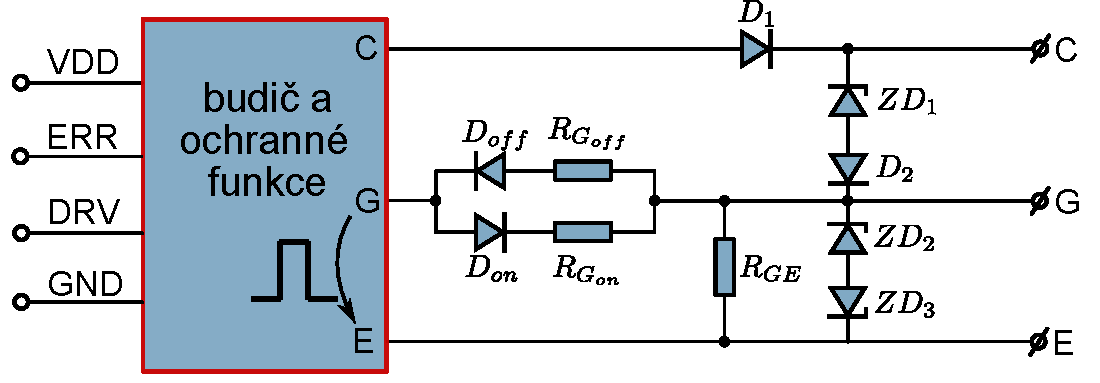
\includegraphics[width=0.7\linewidth]{Resistive_gate_control.pdf}
        \caption{Princip budiče s čistě odporovým řízením spínání společně se
                základními ochranami IGBT}\label{VE:fig_res_gate_drv}
      \end{figure}


      \subsubsection{Řízení spínacího procesu podle strmosti kolektorového proudu (\texttt{dI/dt control})}
        Je-li $U_{GE} = U_{d_{ON}} > U_{GE_{th}}$ je IGBT spínač ve vodivém stavu a pouze celková
        parazitní indukčnost v obvodu zkratového proudu omezuje di/dt kolektorového proudu.
        Doporučovanou možností jak redukovat maximální kolektorový proud $I_{C_{max}}$ a také
        maximální $dI_C/dt\lvert_{max}$ je snížení hradlového napětí $U_{GE}$. Pro odvození
        závislosti strmosti kolektorového proudu na hradlovém napětí vyjděme z náhradního schématu
        dle obr. \ref{VE:fig_eqv_cir_IGBT} a idealizovaných průběhů spínacího a vypínacího procesu
        výkonového spínače dle obrázku *. Kolektorový proud v saturaci je možné vyjádřit vztahem
        \begin{equation}\label{VE:eq_Ic_didt1}
           I_C = g_{m}\cdot(U_{GE}-U_{GE_{th}})
        \end{equation}
        kde $g_{m}$ označuje transkonduktanci, $U_{GE_{th}}$ je prahové napětí (threshold voltage)
        \begin{equation}\label{VE:eq_Ig_CGS}
           I_G = C_{GS}\frac{dU_{GS}}{dt}
        \end{equation}
        \begin{equation}\label{VE:eq_Ig_2}
           \frac{dI_C}{dt} = g_{m}\frac{dU_{GS}}{dt} = \frac{g_m}{C_{GS}}\cdot I_G
        \end{equation}
        Je-li $U_Z>U_{L_{SE}}+ U_{GE}$ pak neprochází proud skrz větev omezovače na obr. 
        \ref{VE:fig_didt} a můžeme sestavit náhradní rovnici dle obr. **. Hradlový proud vyjádříme 
        z rovnice (\ref{VE:eq_Ig_2}) a dosadíme do rov.\ref{VE:eq_Ic_didt2}.
        \begin{equation}\label{VE:eq_Ic_didt2}
           U_{d_{ON}} = (R_{G_{int}}+R_{G_{ext}})I_G + U_{GS} + L_{SE_1}\frac{dI_C}{dt}
        \end{equation}
        \begin{align}\label{VE:eq_Ic_didt3}
           U_{d_{ON}} - U_{GS}&= (R_{G_{int}}+R_{G_{ext}})\frac{C_{GS}}{g_m}\frac{dI_C}{dt} + L_{SE_1}\frac{dI_C}{dt}  \\
           \frac{dI_c}{dt}    &= \frac{U_{d_{ON}} - U_{GS}}{(R_{G_{int}}+R_{G_{ext}})\frac{C_{GS}}{g_m} + L_{SE_1}}
        \end{align}
        \begin{figure}[ht!]
          \centering
          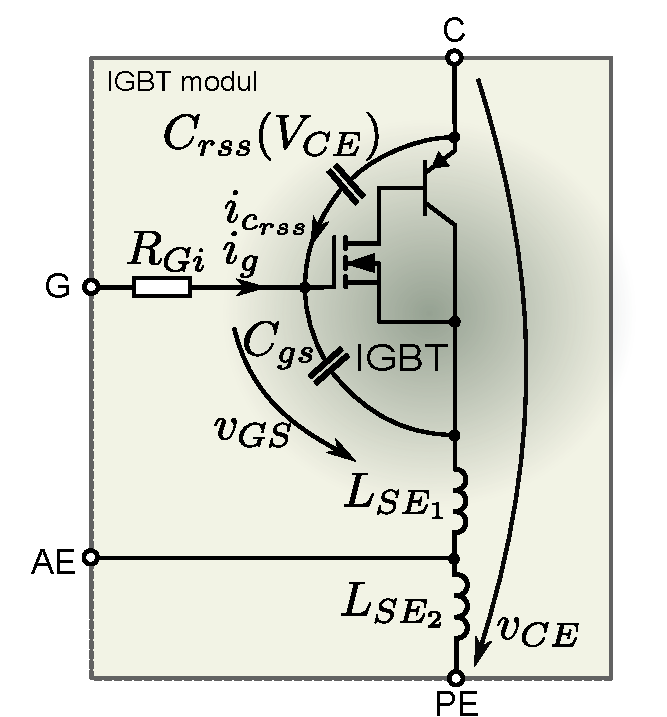
\includegraphics[width=0.6\linewidth]{Eqv_circuit_IGBT_module.pdf}
          \caption{Náhradní schéma IGBT modulu (kapacita $C_{CE}$ a
                   antiparalelní dioda nejsou vyznačeny)}\label{VE:fig_eqv_cir_IGBT}
        \end{figure}

        \begin{figure}[ht!]
          \centering
          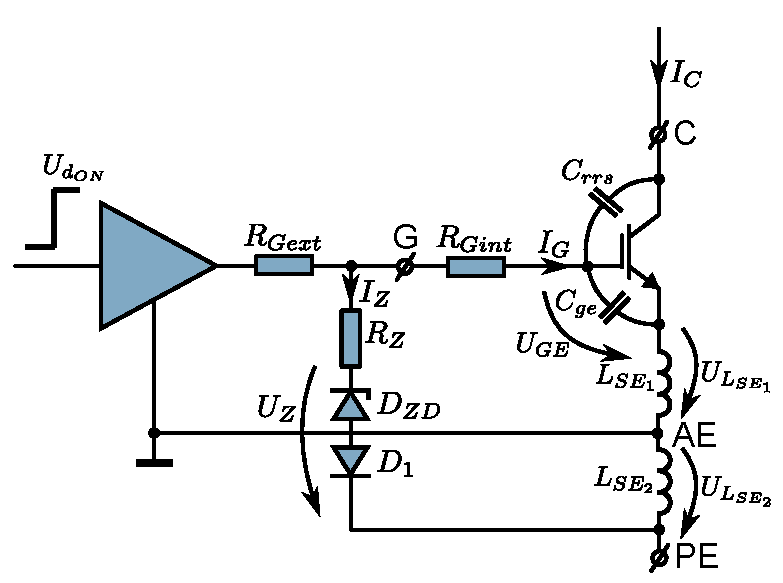
\includegraphics[width=0.9\linewidth]{Eqv_circuit_IGBT_didt.pdf}
          \caption{Obvod budiče se zavedenou zpětnou vazbou od di/dt tvořenou
                   součástkami $R_Z, ZD1, D1$ (kapacita $C_{CE}$ a antiparalelní
                   dioda nejsou vyznačeny)}\label{VE:fig_didt}
        \end{figure}

      \subsubsection{Řízení spínacího procesu podle strmosti kolektorového napětí (\texttt{dU/dt control}) }
        Jednoduchý způsob realizace tohoto způsobu řízení

   \section{Způsoby detekce nadproudu}%SHORT CIRCUIT PROTECTION

     Vysoká spolehlivost provozu výkonového systému, je v současnosti standardním požadavkem 
     moderní komerční aplikace IGBT. Ochrana výkonových prvků před destrukcí v případě nadproudu je 
     tedy nezbytná a bývá řešena následujícími konvenčními metodami:
     \begin{itemize}
       \item hlídání hodnoty kolektorového napětí $U_{CE}$ - collector-emitter voltage monitoring  
             method (viz \ref{PVE:Vce_monitoring}),
       \item proudový transformátor - current transformer (CT).
     \end{itemize}
     První metoda je velice jednoduchá a její princip spočívá ve vyhodnocování úbytku mezi 
     kolektorem a emitorem sepnutého tranzistoru. Problém nastává u vysokonapěťových aplikací, kde 
     je nutné použít vysokonapěťovou signálovou diodu a navíc ochrana nefunguje během přechodného 
     děje spínacího procesu, protože napětí $U_{CE}$ klesá pomalu. Je tedy vhodné používat tuto 
     ochranu v kombinaci s jinou. Širokému použití proudových transformátorů jen pro ochranné účely 
     brání především cena spolu s velkým počtem kusů pro pokrytí všech možných kombinací zkratových 
     obvodů, jež v dané aplikaci mohou nastat.

     Následující kapitoly budou věnovány metodám detekce poruchového stavu a způsobům bezpečného 
     vypnutí IGBT i v těchto nepříznivých režimech. Nejprve bude nutné kategorizovat možné 
     poruchové režimy podle chování IGBT. Zajištění těchto funkcí je náplní moderního budiče IGBT.

     \subsection{Uvažované typy zkratových obvodů ve větvi vý\-ko\-no\-vého měniče s 
     indukční zátěží}
       \begin{figure}[ht!]
         \centering
         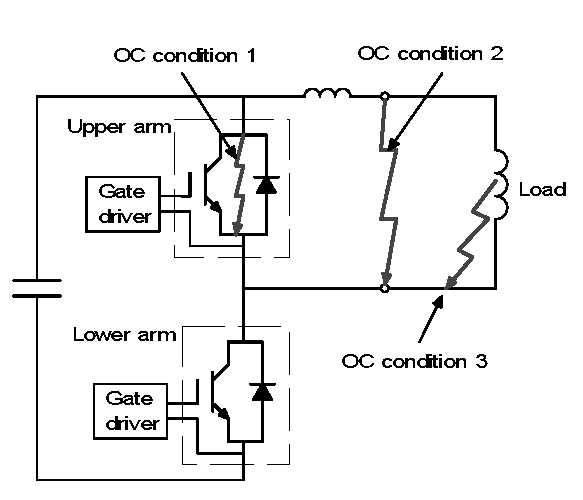
\includegraphics[width=0.7\linewidth]{IGBT_OC_condition.pdf}
         \caption[Kategorie zkratových obvodů]{Znázornění třech uvažovaných zkratových obvodů ve
                  větvi výkonového měniče s indukční zátěží}\label{VE:fig_OC_condition}
       \end{figure}

     \subsection{Monitorování velikosti kolektorového napětí}\label{PVE:Vce_monitoring}
     \subsection{Omezovač hradlového napětí - $V_{GE}\ clamping$}\label{PVE:Vge_clamping}
     \begin{subequations}\label{PVE:eq_Vzge_tranzil}
     \begin{align}
       U_{Z_{GE}}   &=    U_Z\cdot(1+\alpha_T\cdot\Delta\vartheta_j)\cdot(1+T_V)\leq
                          U_{GE_{peak}},                                                      \\
       U_{GE_{max}} &\leq U_Z\cdot(1-T_V)
     \end{align}
     \end{subequations}
     kde: $U_Z\ldots$ jmenovité napětí transilu; $U_{GE_{peak}}\ldots$ špičková hodnota hradlového 
     napě\-tí - při zkratu: $\leq17,5V$; $\alpha_T\ldots$ teplotní koeficient transilu; 
     $\Delta\vartheta_j\ldots$ oteplení nad jmenovitou teplotu okolí 25°C; $T_V\ldots$ katalogová 
     tolerance transilu

       \begin{figure}[ht!]
         \centering
         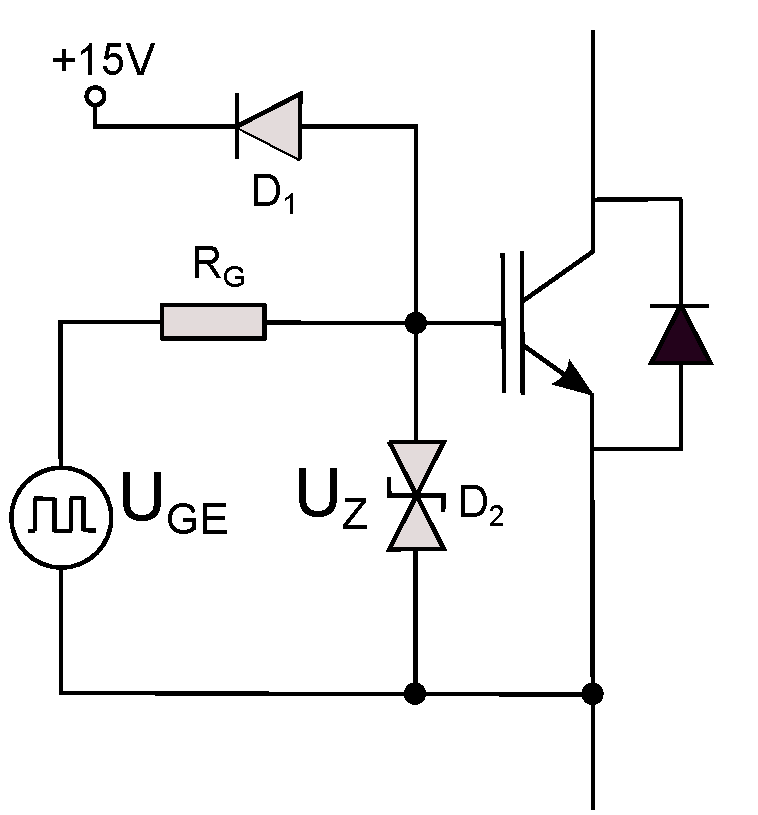
\includegraphics[width=0.4\linewidth]{Vge_clamping.pdf}
         \caption[Omezovač hradlového napětí]{Jednoduchá realizace omezovače
                  hradlového napětí pomocí Shottkyho diody nebo tranzilu}\label{VE:fig_Vge_clamp}
       \end{figure}

     Na obrázku \ref{VE:fig_Vge_clamp} jsou znázorněny dvě jednoduché možnosti. V případě použití
     transilu je nutné dbát zvýšenou pozornost jeho výběru. Průrazné napětí musí mít co nejnižší
     rozptyl a při změně teploty okolí nesmí v běžném provozu omezovat budicí signál. Těmto
     požadavkům nejlépe vyhovuje transil 1.5KE16CA:
      \begin{itemize}
        \item $\alpha_T = 8\cdot10^{-4}\ (12mV/K)$,
        \item $\Delta\vartheta_j = 50K$ (předpoklad),
        \item $T_V = 5\%$,
      \end{itemize}
     z čehož vyplývají následující kontrolní rovnice
      \begin{align}
        U_Z(@+75°C; +5\%) &= 17,53V\approx U_{GE_{peak}}\\
        U_Z(@-25°C; -5\%) &= 14,53V\approx U_{GE_{min}} \\
        U_Z(@+25°C; -5\%) &= 15,20V\geq U_{GE_{max}}
      \end{align}
     V případě krajní hodnoty $U_Z(@-25°C; -5\%)$ dojde při buzení $U_{GE}=\pm15V$ ke krátkodobé
     aktivaci ochranného transilu, což způsobí jeho ohřátí a posunutí hladiny $U_Z$.

     Efektivita varianty se Shottkyho diodou (viz obr.\ref{VE:fig_Vge_clamp}) je závislá na 
     velikosti parazitní indukčnosti mezi hradlem a kondenzátorem zdroje budiče. Zdroj budiče musí 
     také zajistit aby napětí na tomto kondenzátoru při funkci ochrany nevzrůstalo.    

%---------------------------------------------------------------------------------------------------